\documentclass[tikz]{standalone}

\usepackage{mathtools}
\usetikzlibrary{decorations.markings,decorations.pathmorphing}

\let\Im\relax
\DeclareMathOperator{\Im}{Im}
\let\Re\relax
\DeclareMathOperator{\Re}{Re}

\def\xr{3.5}
\def\yr{1.6}

\begin{document}
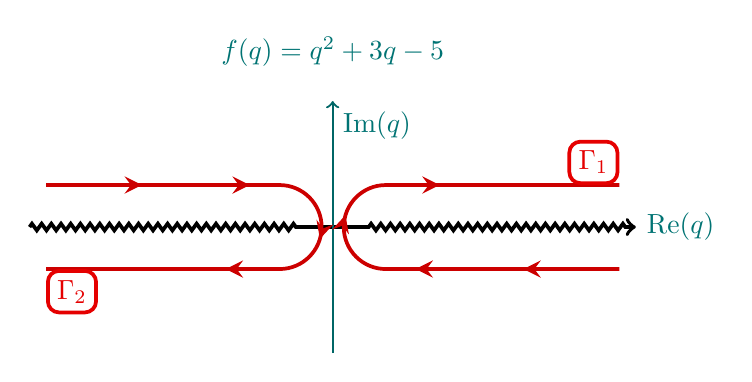
\begin{tikzpicture}[line width=1.35pt]

  % Axes: horizontal zigzag, vertical straight
  \draw [decorate,decoration={zigzag,segment length=3.5,amplitude=1.2,post=lineto,post length=13}] (-1.1*\xr,0) -- (0,0);
  \draw [->,decorate,decoration={zigzag,segment length=3.5,amplitude=1.2,pre=lineto,pre length=13,post=lineto,post length=3}] (0,0) -- (1.1*\xr,0) node [right, teal!90!black] {$\Re(q)$};
  \draw [->,thick,teal!80!black] (0,-\yr) -- (0,\yr) node [below right, teal!90!black] {$\Im(q)$};

  % Left path (Physics contour, with arrows)
  \draw[xshift=4,red!80!black,decoration={markings,mark=between positions 0.16 and 0.84 step 0.18 with {\arrow[scale=1.15]{stealth}}},postaction={decorate}]
    (\xr,-\yr/3) -- (\yr/3,-\yr/3) arc (-90:-270:\yr/3) (\yr/3,\yr/3) -- (\xr,\yr/3) node[above left, red!90!black, rounded corners, draw, fill=white] {$\Gamma_1$};

  % Right path (Physics contour, with arrows)
  \draw[xshift=-4,red!80!black,decoration={markings,mark=between positions 0.16 and 0.84 step 0.18 with {\arrow[scale=1.15]{stealth}}},postaction={decorate}]
    (-\xr,\yr/3) -- (-\yr/3,\yr/3) arc (90:-90:\yr/3) (-\yr/3,-\yr/3) -- (-\xr,-\yr/3) node[below right, red!90!black, rounded corners, draw, fill=white] {$\Gamma_2$};

  % Sample equation annotation (Physics context)
  \node[above, align=center, teal!90!black] at (0, \yr+0.3) {$f(q) = q^2 + 3q - 5$};

\end{tikzpicture}
\end{document}